\section{Rigid Body Spring Model (RBSM)}

The simulations are carried out by the three dimensional RBSM, proposed by Kawai et al.,1978\cite{Kawai}. By using 3D RBSM, a concrete model is meshed into rigid bodies, with each consists six degree of freedoms, shown in Figure \ref{fig:RBSM}.

\begin{figure}[ht!]
\centering
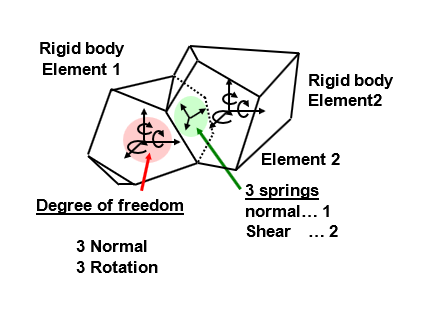
\includegraphics[width=.6\linewidth]{Files/Background/RBSM_1.png}
  \caption{Rigid Body Spring Model[Kohei Nagai et al., 2005\cite{Nagai}]}
  \label{fig:RBSM}
\end{figure}

These six freedoms are three transitional freedoms and three rotational freedoms at the center point within the element, developed by Kohei Nagai et al., 2005\cite{Nagai}.

The computational point $(x_c, y_c, z_c)$ is defined as,

\begin{equation}
  \begin{aligned}
  &x_c=\frac{x_1 + x_2 + \cdots + x_i + \cdots + x_m}{m} \\
  &y_c=\frac{y_1 + y_2 + \cdots + y_i + \cdots + y_m}{m} \\
  &z_c=\frac{z_1 + z_2 + \cdots + z_i + \cdots + z_m}{m}
  \end{aligned}
\end{equation}

where m is the number of node composing an element and $x_i$, $y_i$ and $z_i$ are the coordinates of the nodes in an element.

Three individual springs, which are one normal spring and two shear spring, are set at a point on the face between two elements. This point $(x_{cf}, y_{cf}, z_{cf})$ is defined as,

\begin{equation}
  \begin{aligned}
  &x_{cf}=\frac{x_1 + x_2 + \cdots + x_j + \cdots + x_n}{n} \\
  &y_{cf}=\frac{y_1 + y_2 + \cdots + y_j + \cdots + y_n}{n} \\
  &z_{cf}=\frac{z_1 + z_2 + \cdots + z_j + \cdots + z_n}{n}
  \end{aligned}
\end{equation}

Where m is the number of nodes composing the face and $x_j$, $y_j$ and $z_j$ are those coordinates.

Since cracks initiate and propagate along the boundary face, the mesh arrangement may affect fracture direction. Random geometry is introduced to avoid the formation of cracks in a certain direction by using a Voronoi diagram.

In the nonlinear analysis, a stiffness matrix is constructed based on the principle of virtual work (Kawai and Takeuchi 1990\cite{Kawai}), and the Modified Newton-Raphson method is employed for the convergence algorithm.

When an element has small displacement $[u_1, v_1, w_1, \theta_{u1}, \theta_{v1}, \theta_{w1}]$, the springs at a face in an element will be displaced:

\begin{equation}
  \begin{aligned}
  &u = u_1 - \theta_{w1} (y_{cf} - y_{ce1}) + \theta_{v1} (z_{cf} - z_{ce1}) \\
  &v = v_1 - \theta_{u1} (z_{cf} - z_{ce1}) + \theta_{w1} (x_{cf} - x_{ce1}) \\
  &w = w_1 - \theta_{v1} (x_{cf} - x_{ce1}) + \theta_{u1} (y_{cf} - y_{ce1})
  \end{aligned}
\end{equation}

Elongations of normal and shear spring are calculated and expressed as:

\begin{equation}
  d = Bu_e
\end{equation}

where $d^T = [\delta_{s1}, \delta_{s2}, \delta_n]$ and $u_e^T = [u_1, v_1, w_1,\theta_{u1}, \theta_{v1}, \theta_{w1}, u_2, v_2, w_2,\theta_{u2}, \theta_{v2}, \theta_{w2}]$

The transformation matrix B is written as:

\begin{equation}
  B =
  \begin{vmatrix}
    K_{11} &K_{12} &K_{13} &K_{14} &{\cdots} &K_{19} &K_{110} &K_{111} &K_{112}\\
    K_{21} &K_{22} &K_{23} &K_{24} &{\cdots} &K_{29} &K_{210} &K_{211} &K_{212}\\
    K_{31} &K_{32} &K_{33} &K_{34} &{\cdots} &K_{39} &K_{310} &K_{311} &K_{312}
  \end{vmatrix}
\end{equation}

where \\
$K_{11} = -e_{s1x}$    $K_{21} = -e_{s2x}$    $K_{31} = -e_{nx}$ \\
$K_{12} = -e_{s1y}$    $K_{22} = -e_{s1y}$    $K_{32} = -e_{ny}$ \\
$K_{13} = -e_{s1z}$    $K_{23} = -e_{s2z}$    $K_{33} = -e_{nz}$ \\
\\
$K_{14} = e_{s1y}(z_{cf}-z{ce1})-e_{s1z}(y_{cf}-y_{ce1})$\\
$K_{24} = e_{s2y}(z_{cf}-z{ce1})-e_{s2z}(y_{cf}-y_{ce1})$\\
$K_{34} = e_{ny}(z_{cf}-z{ce1})-e_{nz}(y_{cf}-y_{ce1})$\\
\\
$K_{15} = e_{s1z}(x_{cf}-x{ce1})-e_{s1x}(z_{cf}-z_{ce1})$\\
$K_{25} = e_{s2z}(x_{cf}-x{ce1})-e_{s2x}(z_{cf}-z_{ce1})$\\
$K_{35} = e_{nz}(x_{cf}-x{ce1})-e_{nx}(z_{cf}-z_{ce1})$\\
\\
$K_{15} = e_{s1z}(x_{cf}-x{ce1})-e_{s1x}(z_{cf}-z_{ce1})$\\
$K_{25} = e_{s2z}(x_{cf}-x{ce1})-e_{s2x}(z_{cf}-z_{ce1})$\\
$K_{35} = e_{nz}(x_{cf}-x{ce1})-e_{nx}(z_{cf}-z_{ce1})$\\
\\
$K_{16} = e_{s1x}(y_{cf}-y{ce1})-e_{s1y}(x_{cf}-x_{ce1})$\\
$K_{26} = e_{s2x}(y_{cf}-y{ce1})-e_{s2y}(x_{cf}-x_{ce1})$\\
$K_{36} = e_{nx}(y_{cf}-y{ce1})-e_{ny}(x_{cf}-x_{ce1})$\\
\\
$K_{17} = e_{s1x}$    $K_{27} = e_{s2x}$    $K_{37} = e_{nx}$ \\
$K_{18} = e_{s1y}$    $K_{28} = e_{s1y}$    $K_{38} = e_{ny}$ \\
$K_{19} = e_{s1z}$    $K_{29} = e_{s2z}$    $K_{39} = e_{nz}$ \\
\\
$K_{110} = e_{s1z}(y_{cf}-y{ce2})-e_{s1y}(z_{cf}-z_{ce2})$\\
$K_{210} = e_{s2z}(y_{cf}-y{ce2})-e_{s2y}(z_{cf}-z_{ce2})$\\
$K_{310} = e_{nz}(y_{cf}-y{ce2})-e_{ny}(z_{cf}-z_{ce2})$\\
\\
$K_{111} = e_{s1x}(z_{cf}-z{ce2})-e_{s1z}(x_{cf}-x_{ce2})$\\
$K_{211} = e_{s2x}(z_{cf}-z{ce2})-e_{s2z}(x_{cf}-x_{ce2})$\\
$K_{311} = e_{nx}(z_{cf}-z{ce2})-e_{nz}(x_{cf}-x_{ce2})$\\
\\
$K_{112} = e_{s1y}(x_{cf}-x{ce2})-e_{s1x}(y_{cf}-y_{ce2})$\\
$K_{212} = e_{s2y}(x_{cf}-x{ce2})-e_{s2x}(y_{cf}-y_{ce2})$\\
$K_{312} = e_{ny}(x_{cf}-x{ce2})-e_{nx}(y_{cf}-y_{ce2})$\\

where $e_{ij}$ is direction cosine in i axis on j axis.

By applying the principal of virtual work, the local equilibrium relation expressed in global coordinate is:

\begin{equation}
  k_e \delta u_e = \delta f_e
\end{equation}

where the stiffness associated with interconnected face $k_e$ is given as:

\begin{equation}
  k_e = B^T DB
\end{equation}

where
\begin{equation}
  D = \begin{vmatrix}
        k_{s1} &0 &0 \\
        0 &k_{s2} &0 \\
        0 &0 &k_3
      \end{vmatrix}
\end{equation}

in which $k_n$, $k_{s1}$, and $k_{s2}$ are the normal and shear spring stiffness. $k_n$, $k_{s1}$, and $k_{s2}$ can be calculated as:
\begin{equation}
  \begin{aligned}
    &k_n = k_{sp} \frac{A}{h_1 + h_2} \\
    &k_{s1} = k_{ssp} \frac{A}{h_1 + h_2} \\
    &k_{s2} = k_{ssp} \frac{A}{h_1 + h_2}
  \end{aligned}
\end{equation}

where

\begin{equation}
  \begin{aligned}
    &k_{nsp} = \frac{(1-\theta_{elem})E_{elem}}{(1+\theta_{elem})(1-2\theta_{elem})} \\
    &k_{ssp} = \frac{E_{elem}}{1+\theta_{elem}}
  \end{aligned}
\end{equation}

where $h_1$ and $h_2$ are length of perpendicular lines from the element computational point to the face where springs are set.

$E_{elem}$ and $v_{elem}$ are the modulus of elasticity and poison's ratio, respectively:

\begin{equation}
  \begin{aligned}
    &E_{elem} = \frac{E_{elem1} h_1 + {E_{elem2} h_2}}{h_1+h_2} \\
    &\theta_{elem} = \frac{\theta_{elem1} h_1 + {\theta_{elem2} h_2}}{h_1+h_2}
  \end{aligned}
\end{equation}

In the convergence process, displacements that cancel the unbalanced force of elements are added to the elements.

The displacements are calculated using the stiffness matrix. Convergence of the model is judged when the ratio of
$\sum_{} $(Unbalanced force of element in the model)$^2$ to \\
$\sum_{} $(Applied force to element)$^2$ becomes less than $10^5$.
%*******10********20********30********40********50********60********70********80

%*******10********20********30********40********50********60********70********80
\section{Rigid Body Spring Model (RBSM)}

A constitutive model for the concrete part at the mesoscale is used in this research since constitutive model in the macro scale cannot be applied to the mesoscale analysis.

In the analysis, the values of the material properties at the meso level given to the elements are actually different from the material properties where the object is analyzed at the macroscopic scale.

The material properties for the elements were determined to give the correct macroscopic properties.  In the discrete analysis done by Nagai et al. in 2005, the shape and fineness of elements do affect the analysis results.

As we concern that the crack direction may affect the crack pattern, size of each concrete elements should be under consideration. Here for small example using 10x10x10mm model, the average diameter of elements is selected to be 0.05mm, while for larger size model in the dimension of 100x100x100mm, the size of each element is approximately 2x2x2mm to 3x3x3mm, almost the size of smallest coarse aggregate introduced. This assumption was made to represent the fracture behavior in concrete in a relatively high fineness and the behavior of both mortar and aggregate can be well presented.

In the elastic analysis, the relationship between macroscopic and mesoscopic Poisson's ratio, the effect of the mesoscopic Poisson's ratio on the macroscopic elastic modulus, are all confirmed by Nagai et al. in 2005, using the same concepts.

\begin{equation}
  \begin{aligned}
  &\theta_{elem} = -24.8\theta^4+31.9\theta^3-16.4\theta^2 +4.28\theta\\
  &E_{elem} = (-33.7\theta_{elem}^4 + 17.0\theta_{elem}^3 - 4.13\theta_{elem}^2 + 0.327\theta_{elem} + 1)E
  \end{aligned}
\end{equation}

where E and $\theta$ are the macroscopic elastic modulus and Poisson's ratio of the analysis object, respectively.

The material characteristics of each component are presented by means of modeling springs. In normal spring, compressive and tensile stress ($\sigma$) are developed. Shear stress($\tau$) are developed by shear springs.

The elastic modulus of normal sprint($k_{nsp}$ and $k_{ssp}$) was presented in the previous chapter. For calculation of shear stress on 3D analysis, a resultant value of strains generated in two shear springs is adopted as shear strain in the constitutive model presented in this chapter. The strains and stress are calculated as follows:

\begin{equation}
  \begin{aligned}
  &\varepsilon = \frac{\delta_n}{h_1 + h_2}\\
  &\gamma = \frac{\delta_s}{h_1 + h_2}\\
  &\sigma = k_{nsp}\varepsilon\\
  &\tau = k_{ssp}\gamma
  \end{aligned}
\end{equation}

where $\varepsilon$ and $\gamma$ are the strain of normal and shear springs, respectively. $\delta_n$ and $\delta_s$ are the normal and shear relative displacement of elements of those springs, respectively.

In this study, the constitutive model of the concrete element has been developed based on simulations in material scale level. The constitutive models for the normal and shear springs of the concrete elements are shown in Figure %TODO:\ref{}.

%TODO: EDDY P32

The constitutive models of normal spring and a shear spring of concrete element using in this research are shown in Figure %TODO: \ref{}.

Basically, the concept of the concrete model is the same as the original simulation development by Nagai et al., 2005, where the compressive failure is not allowed at the mesoscale. In the tension zone, crack between two rigid bodies occurs only when the tensile stress of the normal spring exceeds the tensile strength of the concrete($f_t$). After exceeding the tensile strength($f_t$), the tensile stress of a normal spring is assumed to decrease bi-linearly, depending on the crack width, to zero at the maximum crack width($w_{max}$), which here is assumed as 0.3mm. An elasto-plastic behavior is also assumed when coming to the shear spring of concrete element with the$\tau_{max}$ is calculated based on the following equations:

\begin{equation}
  \begin{aligned}
  &\tau_{max} = \pm (1.6f_{telem}^2 (-\sigma + f_{telem})^0.4 + 0.15f_{telem}) if (\sigma \geq 3f_{telem})\\
  &\tau_{max} = \pm (1.6f_{telem}^2 (-3f_{telem} + f_{telem})^0.4 + 0.15f_{telem}) if (\sigma < 3f_{telem})
  \end{aligned}
\end{equation}

Besides, if fracture occurs in the normal spring, the calculated shear stress will be reduced according to the reduction of the normal stress. As a result, shear spring will now abole to carry the stress any longer when the crack width of the normal spring reaches $w_{max}$.


% \subsection{Mortar Model}
%
% In this study, constitutive model for concrete at meso scale is developed because constitutive model at the  macro scale cannot be applied directly to meso scale analysis.
%
% The material characteristics of each component are presented by means of modeling spring.
%
% PIC Constitutive models of concrete
%
% In normal springs, compressive and tensile stresses ($\theta$) are developed. Shear springs develop shear stress ($\tau$). The elastic modulus of normal spring ($k_n$) and shear spring ($k_s$) are presented assuming a plane strain condition, where kn and ks are the elastic modulus of normal and shear spring, and $E_{elem}$ and $v_{elem}$ are the corrected elastic modulus and Poisson’s ratio of component at the meso scale, respectively.
%
% \begin{equation}
%   \begin{aligned}
%    &\theta_{elem} = -24.8\theta^4 + 31.9\theta^3 - 16.4\theta^2 + 4.28\theta \\
%    &E_{elem} = (-33.7\theta_{elem}^4 + 17.0\theta_{elem}^3 - 4.13\theta^2 + 0.327\theta_{elem}+1)E
%   \end{aligned}
% \end{equation}
%
% For calculation of shear stress, a resultant value of strains generated in two shear springs is adopted as a shear strain in the constitutive model presented in this chapter.
%
% \begin{equation}
%   \begin{aligned}
%    &\varepsilon = \frac{\delta_n}{h_1+h_2} \\
%    &\gamma = \frac{\delta_s}{h_1+h_2} \\
%    &\sigma = k_{nsp}\varepsilon \\
%    &\tau = k_{ssp}\gamma
%   \end{aligned}
% \end{equation}
%
% \subsection{Aggregate Model}
%
% In this study, the effect of the existence of aggregate in
% concrete on the fracture process is examined. For this
% purpose, aggregate elements are assumed to behave only
% elastically without fracture in this study.
%
% The same equations as (3?), (4?), (5?) and (7?) are adopted to present the material property of aggregate.
%
% Pic Of AGGREGATE
